
\documentclass[9pt,conference]{IEEEtran}

% *** CITATION PACKAGES ***
\usepackage{cite}

% *** GRAPHICS RELATED PACKAGES ***
\usepackage[pdftex]{graphicx}
\graphicspath{{../figures}}
\DeclareGraphicsExtensions{.pdf}
\usepackage[font=small, labelfont=bf, format=plain, labelsep=space, figurename=Figure, tablename=Table]{caption}\usepackage[labelfont=rm, labelformat=parens, labelsep=space]{subcaption}

% *** MATH PACKAGES ***
\usepackage[cmex10]{amsmath}
\usepackage{amssymb}
\usepackage{bm}

% *** SPECIALIZED LIST PACKAGES ***
\usepackage{siunitx}
\sisetup{detect-all=true, detect-family=true}

% *** MISC PACKAGES ***
\usepackage{color}

\begin{document}
%
% paper title
% can use linebreaks \\ within to get better formatting as desired
\title{A compressed-sensing approach for ultrasound imaging}

\author{\IEEEauthorblockN{Adrien Besson\IEEEauthorrefmark{1},
		Rafael E. Carrillo\IEEEauthorrefmark{2}, 
		Dimitris Perdios\IEEEauthorrefmark{1},
		Marcel Arditi\IEEEauthorrefmark{1},
		Yves Wiaux\IEEEauthorrefmark{3}, and 
	Jean-Philippe Thiran\IEEEauthorrefmark{1}\IEEEauthorrefmark{4}}
	\IEEEauthorblockA{\IEEEauthorrefmark{1}Signal Processing Laboratory (LTS5),
		Ecole Polytechnique F\'{e}d\'{e}rale de Lausanne,
		Lausanne, Switzerland\\}
	\IEEEauthorblockA{\IEEEauthorrefmark{2}Centre Suisse d'Electronique et de Microtechnique~(CSEM), Neuch\^atel, Switzerland\\}
	\IEEEauthorblockA{\IEEEauthorrefmark{3}Institute of Sensors, Signals and Systems, Heriot-Watt University, Edinburgh, United-Kingdom\\}
	\IEEEauthorblockA{\IEEEauthorrefmark{4}Department of Radiology, University Hospital Center (CHUV) and University of Lausanne (UNIL), Lausanne, Switzerland}}
\maketitle

% conference papers do not typically use \thanks and this command
% is locked out in conference mode. If really needed, such as for
% the acknowledgment of grants, issue a \IEEEoverridecommandlockouts
% after \documentclass

% for over three affiliations, or if they all won't fit within the width
% of the page, use this alternative format:
% 
%\author{\IEEEauthorblockN{Michael Shell\IEEEauthorrefmark{1},
%Homer Simpson\IEEEauthorrefmark{2},
%James Kirk\IEEEauthorrefmark{3}, 
%Montgomery Scott\IEEEauthorrefmark{3} and
%Eldon Tyrell\IEEEauthorrefmark{4}}
%\IEEEauthorblockA{\IEEEauthorrefmark{1}School of Electrical and Computer Engineering\\
%Georgia Institute of Technology,
%Atlanta, Georgia 30332--0250\\ Email: see http://www.michaelshell.org/contact.html}
%\IEEEauthorblockA{\IEEEauthorrefmark{2}Twentieth Century Fox, Springfield, USA\\
%Email: homer@thesimpsons.com}
%\IEEEauthorblockA{\IEEEauthorrefmark{3}Starfleet Academy, San Francisco, California 96678-2391\\
%Telephone: (800) 555--1212, Fax: (888) 555--1212}
%\IEEEauthorblockA{\IEEEauthorrefmark{4}Tyrell Inc., 123 Replicant Street, Los Angeles, California 90210--4321}}




% use for special paper notices
%\IEEEspecialpapernotice{(Invited Paper)}




% make the title area
\maketitle


\begin{abstract}
%\boldmath
Ultrasonography uses multiple piezoelectric element probes to image tissues. Current time-domain beamforming techniques require the signal at each transducer-element to be sampled at a rate higher than the Nyquist criterion, resulting in an extensive amount of data to be received, stored and processed. In this work, we propose to exploit sparsity of the signal received at each transducer-element. The proposed approach uses multiple compressive multiplexers for signal encoding and solves an $\ell_1$-minimization in the decoding step, resulting in the reduction of \SI{75}{\percent} of the amount of data, the number of cables and the number of analog-to-digital converters required to perform high quality reconstruction.
\end{abstract}
% IEEEtran.cls defaults to using nonbold math in the Abstract.
% This preserves the distinction between vectors and scalars. However,
% if the conference you are submitting to favors bold math in the abstract,
% then you can use LaTeX's standard command \boldmath at the very start
% of the abstract to achieve this. Many IEEE journals/conferences frown on
% math in the abstract anyway.

% no keywords




% For peer review papers, you can put extra information on the cover
% page as needed:
% \ifCLASSOPTIONpeerreview
% \begin{center} \bfseries EDICS Category: 3-BBND \end{center}
% \fi
%
% For peerreview papers, this IEEEtran command inserts a page break and
% creates the second title. It will be ignored for other modes.
\IEEEpeerreviewmaketitle
Medical ultrasonography is a widely used modality nowadays due to its non-invasiveness and real-time capability. In many ultrasound~(US) systems, an array of transducer-elements is used to transmit acoustic pulses, which, when reflected back by the medium inhomogeneities, are sensed by the same array. According to the Shannon-Nyquist theorem, the sampling rate at each element must be at least twice the bandwidth of the received signal. In practice, time-domain beamforming techniques require sampling rates between 3 and 10 times the center frequency to minimize the delay-quantization errors~\cite{szabo2014}. Such sampling rates induce high-power requirements for the analog to digital converters and a high data communication bandwidth that are not always achievable in challenging environments.

%The large number of transducer-elements and the high central frequency required in medical ultrasonography motivate the research towards sampling rate reduction.

Let us consider a US probe made of $N_{el}$ transducer-elements and call $r_i \left(t\right)$ with $i \in \left\lbrace 1,...,N_{el}\right\rbrace$ the corresponding echo signals received by each transducer-element at time $t$. If we consider a medium made of $K$ inhomogeneities, then $r_i\left(t\right)~=~\sum_{k=1}^{K} a_{ik} \psi \left(t - t_{k}\right)$, with $\left(a_{ik}, t_{k}\right)$ amplitudes and times-of-arrival of the $K$ echo-pulses to the $i^{th}$ transducer-element and $\psi \left(t\right)$ the elementary waveform. Assuming a linear propagation, we can state that $\psi \left(t\right)~=~\left(e \ast h_{Tx} \ast h_{Rx}\right) \left(t\right)$ where $e\left(t\right)$ denotes the excitation and $ h_{Tx}\left(t\right)$ and $ h_{Rx}\left(t\right)$ are the transmit and receive impulse responses of the transducer-elements, respectively.
Given the model described above, it can be stated that the vector $\bm{r}_i~=~ \left[r_i \left(t_1\right), ..., r_i \left(t_{N_t}\right)\right]^T~\in~ \mathbb{R}^{N_t}$, where $N_t$ denotes the number of time samples, obeys a $K$-sparse synthesis model in an overcomplete dictionary $\mathsf{\Psi} \in \mathbb{R}^{N_t \times N_t}$ made of all the shifted replicas of the pulse~\cite{naini2009}. Thus, $\bm{r}_i = \mathsf{\Psi} \bm{a}_i$ with $\| \bm{a}_i \|_0 = K$, which can be exploited under the compressed sensing~(CS) framework. 
%where the following problem is solved:
%\begin{equation}
%\label{eq_single_channel_problem}
%\min_{\bar{\bm{\alpha_i}}\in\mathbb{R}^{N_t}} || \bar{\bm{\alpha_i}} ||_1
%\textnormal{ subject to }\| \bm{y_i}-\mathsf{\Phi} \mathsf{\Psi}\bar{\bm{\alpha_i}}\|_{2}\leq\epsilon,
%\end{equation}
%where $\mathsf{\Phi} \in \mathbb{R}^{M \times N_t}$ is the sensing matrix and $\bm{y_i} = \mathsf{\Phi}\bm{r_i}$.
Many efforts have been made in order to provide sub-Nyquist acquisition systems which result in different CS architectures such as the Random Demodulator~\cite{tropp2010} and the Random-Modulator Pre-Integrator~\cite{becker2011} for single-channel signals, and the compressive multiplexer for multi-channel signals~\cite{slavinsky2011,kim2012}.
In US imaging, Chernyakova \textit{et al.} have recently proposed a hardware architecture based on finite rate of innovation and Xampling ideas~\cite{chernyakova2014}.

In this work, we propose a proof of concept for a compressive multiplexer~(CMUX) applied to US imaging. The architecture, denoted as US-CMUX is derived from the work of Kim~\textit{et al.}~\cite{kim2012} which have applied CMUX to speech signals. The idea is to split the $N_{el}$ channels of the US probe into $L$ groups of $M$ channels and to mix each group using CMUX. In the decoding step, a convex problem is solved.
The CMUX, described on Figure~\ref{fig:CMUX}, is based on modulating each channel $r_i \left(t\right)$ of a given group by a chipping sequence $p_i \left(t\right)$ sampled from a Rademacher distribution. The modulated channels are then summed to $y \left(t\right)~=~ \sum_{i=1}^{M} p_i \left(t\right) r_i \left(t\right)$ and sampled at $f_s$. 

The US-CMUX, described on Figure~\ref{fig:USCMUX}, uses $L$ CMUX sharing the same chipping sequences to perform the signal encoding, giving rise to the matrix $ \mathsf{Y} = \left[\bm{y_1}, ..., \bm{y_L}\right] \in \mathbb{R}^{N_t \times L}$. In the decoding step, the following convex problem is solved:
\begin{equation}
\label{eq_CMUX_problem}
\min_{\bar{\mathsf{A}} \in \mathbb{R}^{MN_t \times L}} \lVert \bar{\mathsf{A}} \lVert_{11}
\textnormal{ subject to } \| \mathsf{Y}- \mathsf{\Psi}_{P}\bar{\mathsf{A}}\|_F\leq\epsilon,
\end{equation}
where $\|.\|_{11}$ accounts for the $\ell_{11}$-norm, $\|.\|_F$ is the Frobenius norm, $\mathsf{\Psi}_{P}~=~\left[\mathsf{\Psi}_{p1}, ..., \mathsf{\Psi}_{pM}\right] \in \mathbb{R}^{N_t \times M N_t}$ in which $\mathsf{\Psi}_{pi}~=~\left[\bm{p}_i \otimes \Psi_1, ..., \bm{p}_i \otimes \Psi_{N_t}\right] \in \mathbb{R}^{N_t \times N_t}$, where $\otimes$ denotes the Hadamard product, and
\begin{equation*}
\mathsf{A}=
\begin{bmatrix}
\bm{a}_1 & \bm{a}_{M+1} & \dotsb & \bm{a}_{N_{el}-M+1}\\
\vdots & \vdots & & \vdots \\
\bm{a}_M & \bm{a}_{2M} & \dotsb &\bm{a}_{N_{el}} \\
\end{bmatrix} \in \mathbb{R}^{MN_t \times L},
\end{equation*}
 with $\bm{a}_i \in \mathbb{R}^{N_t}$ the representation coefficients of $\bm{r}_i$.
The use of the $\ell_{11}$-norm instead of $\ell_{12}$-norm is motivated by the absence of group sparsity in the problem. Problem~\eqref{eq_CMUX_problem} is solved using the primal-dual forward backward algorithm~\cite{combettes2014}.

In order to validate the proposed method, we present results on an \textit{in-vitro} hyperechoic inclusion phantom~(Model 54GS, CIRS Inc., Norfolk, USA) and an \textit{in-vivo} carotid acquired with a Verasonics research scanner~(V1-128, Verasonics Inc., Redmond, WA). The US probe used for the different experiments is a L12-5~\SI{50}{\milli\metre} probe, with 128 active transducer-elements, working at \SI{5}{\mega\hertz} with \SI{100}{\percent} bandwidth. The sampling frequency is \SI{31.2}{\mega\hertz}, corresponding to 4 times the bandwidth. 
In the proposed work, the element-raw data are firstly acquired with the US system at full rate and the compression is achieved in a post-processing stage using MATLAB. The hardware implementation of the US-CMUX and its constraints are let for future work. The architecture is tested for $L = 2, 4$ which means a reduction of \SI{50}{\percent} and \SI{75}{\percent} of the sampling rate, respectively. In the decoding process, $\epsilon$ is set to $10^{-6}~\|\mathsf{Y}\|_F$ and \num{1500} iterations of the algorithm are run. 
Radio-frequency images are computed with a classical delay-and-sum~(DAS) algorithm, with a linear interpolation for the delay calculation, and the B-mode image is obtained by Hilbert demodulation, normalization and log-compression with a dynamic range of \SI{40}{\decibel}.

The performance of the proposed method is quantified by the signal-to-noise ratio~(SNR) and the structural similarity index~(SSIM) against the computed image using \SI{100}{\percent} of the data, calculated on the B-mode image without log-compression. The results, displayed on Table~\ref{tab:SNR_SSIM}, as well as a visual evaluation on Figures~\ref{fig:anechoic} and~\ref{fig:carotid} show that the proposed architecture leads to high quality reconstruction with \SI{25}{\percent} of the data. 

\begin{figure}[htb]
	\centering
	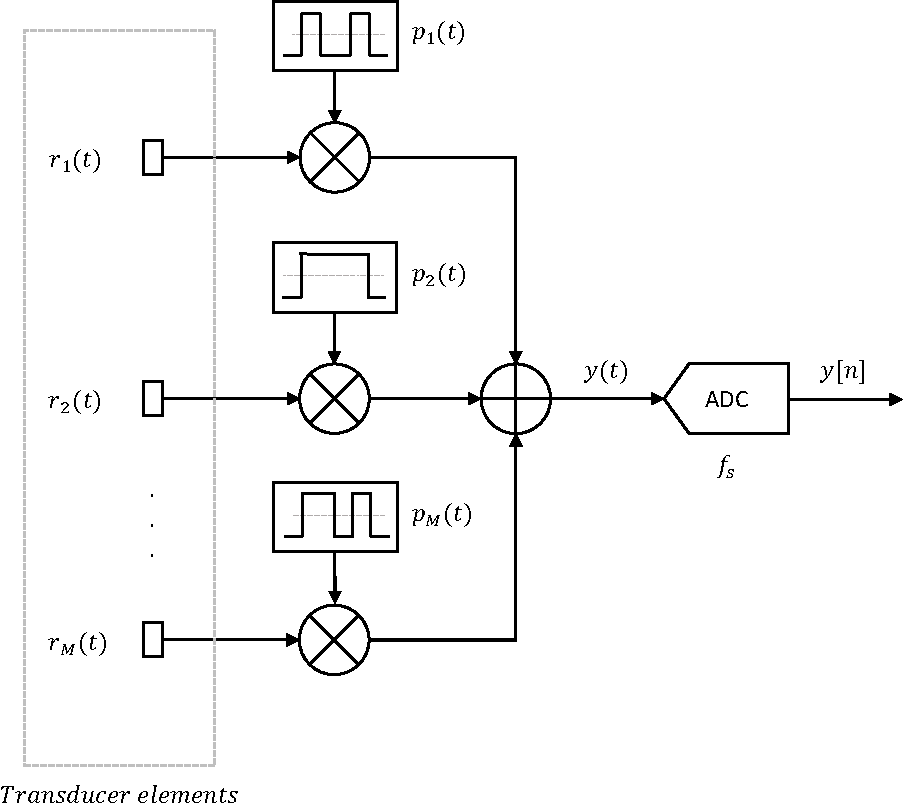
\includegraphics[scale = 0.4]{figures/CMUX.pdf}
	\caption{Compressive multiplexer~(CMUX) architecture for $M$ transducer-elements.}
	\label{fig:CMUX}
\end{figure}
\begin{figure}[htb]
	\centering
	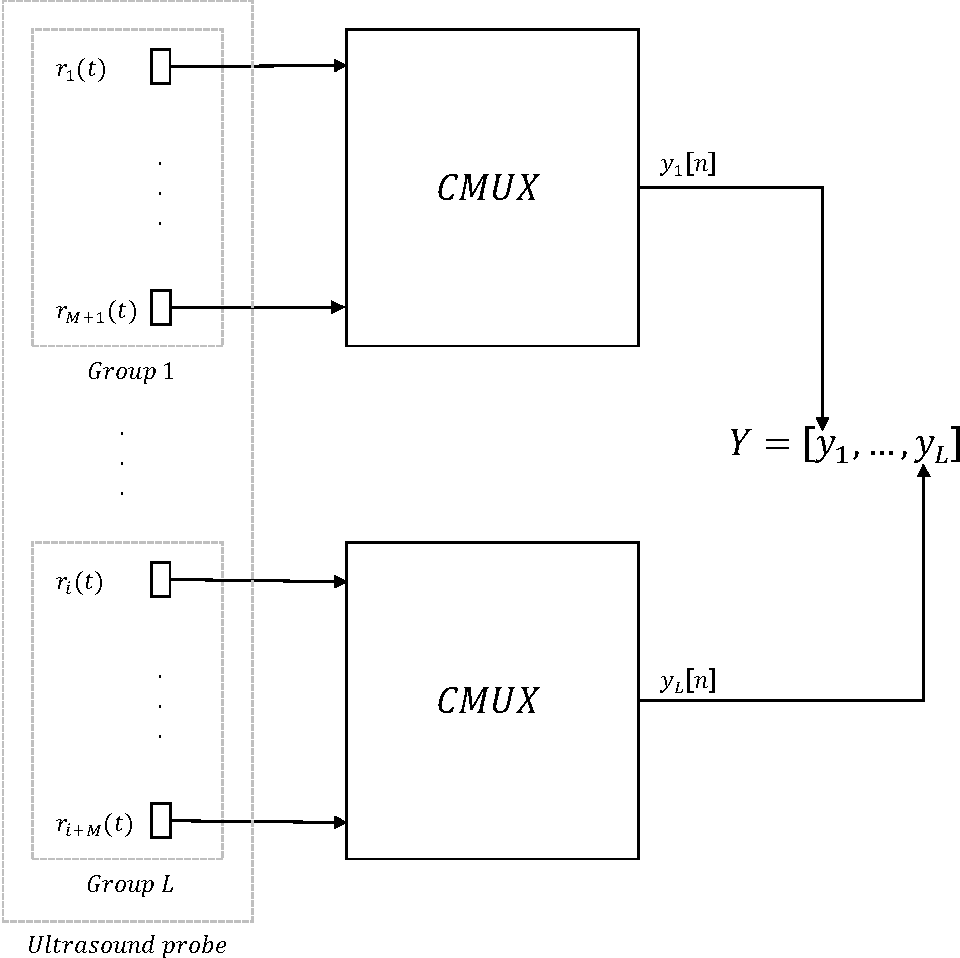
\includegraphics[scale = 0.4]{figures/USCMUX.pdf}
	\caption{Ultrasound compressive multiplexer architecture using $L$ CMUX.}
	\label{fig:USCMUX}
\end{figure}
\newlength{\CarotidFigWidth} \setlength{\CarotidFigWidth}{0.24\textwidth}
\newlength{\CarotidFigHeight}
\settoheight{\CarotidFigHeight}{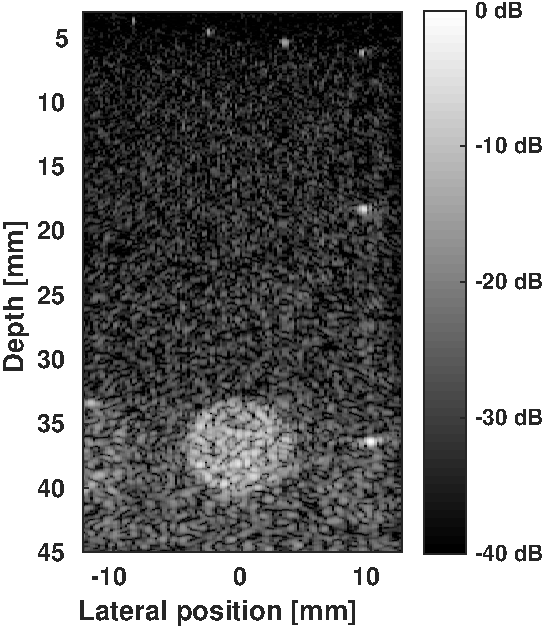
\includegraphics[width=\CarotidFigWidth]{figures/CS_hyperechoic.pdf}} 
\begin{figure}[htb]
	% Maximum length
	\hfill%
	\subcaptionbox{Reference }{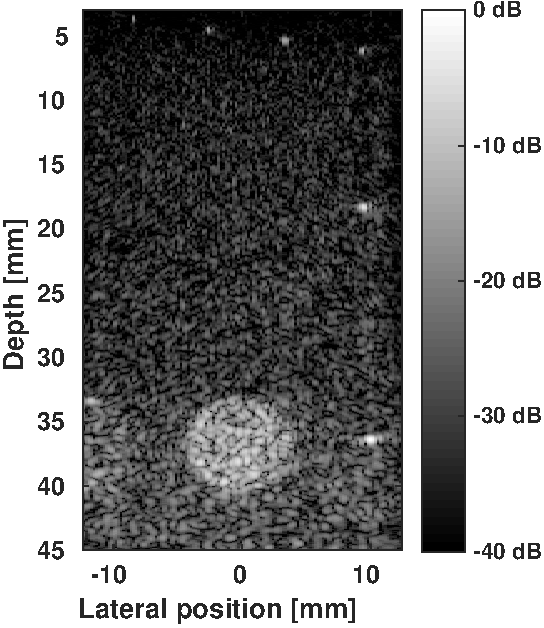
\includegraphics[height=\CarotidFigHeight]{figures/Reference_hyperechoic.pdf}}\hfill%
	\subcaptionbox{CS reconstruction }{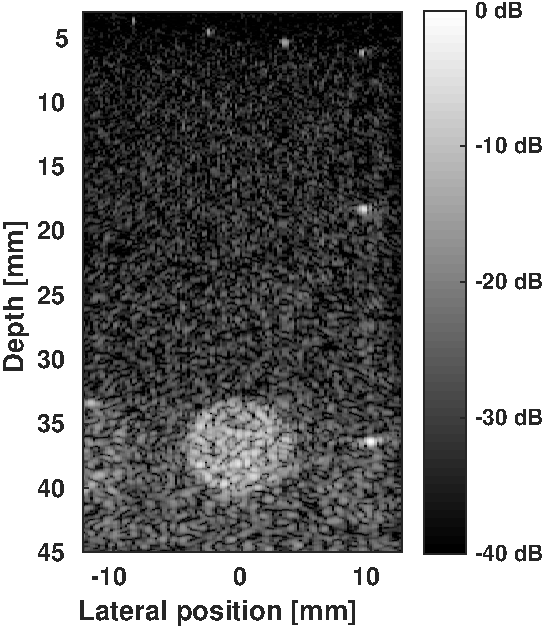
\includegraphics[height=\CarotidFigHeight]{figures/CS_hyperechoic.pdf}}\hfill%
	\caption{B-mode image of the hyperechoic inclusion reconstructed with (a) \SI{100}{\percent} of the data and (b) \SI{25}{\percent} of the data acquired with the US-CMUX architecture.}
	\label{fig:anechoic}
\end{figure}
\setlength{\CarotidFigWidth}{0.24\textwidth}
\settoheight{\CarotidFigHeight}{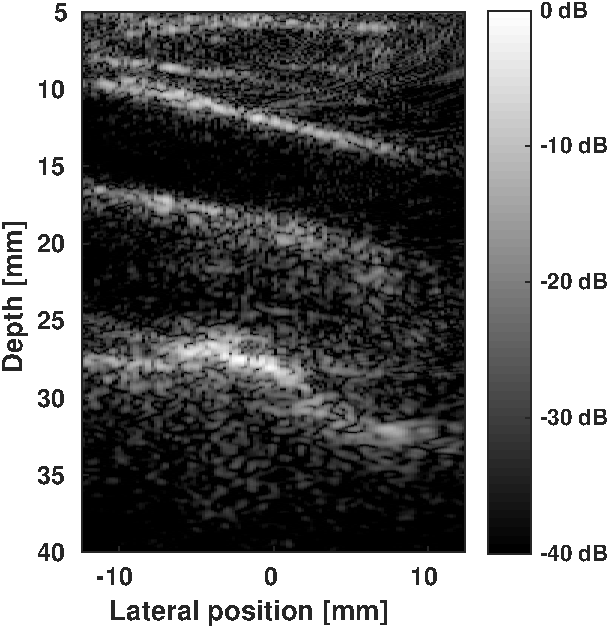
\includegraphics[width=\CarotidFigWidth]{figures/CS_carotid.pdf}}
\begin{figure}[htb]
	% Maximum length
	\hfill%
	\subcaptionbox{Reference }{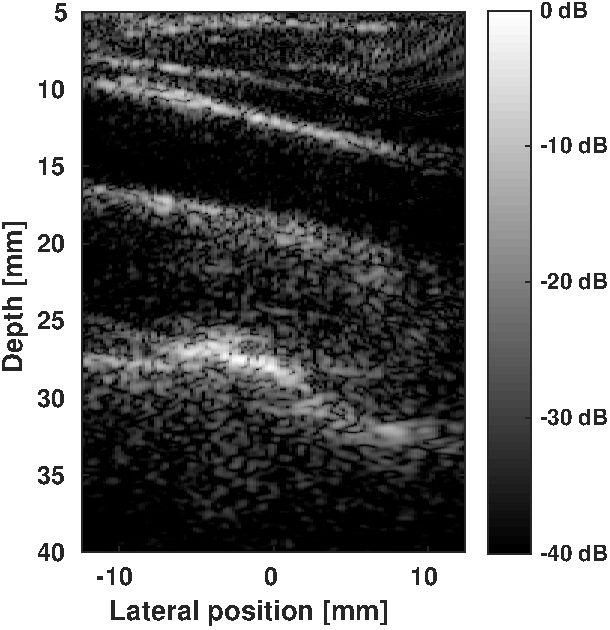
\includegraphics[height=\CarotidFigHeight]{figures/Reference_carotid.pdf}}\hfill%
	\subcaptionbox{CS reconstruction }{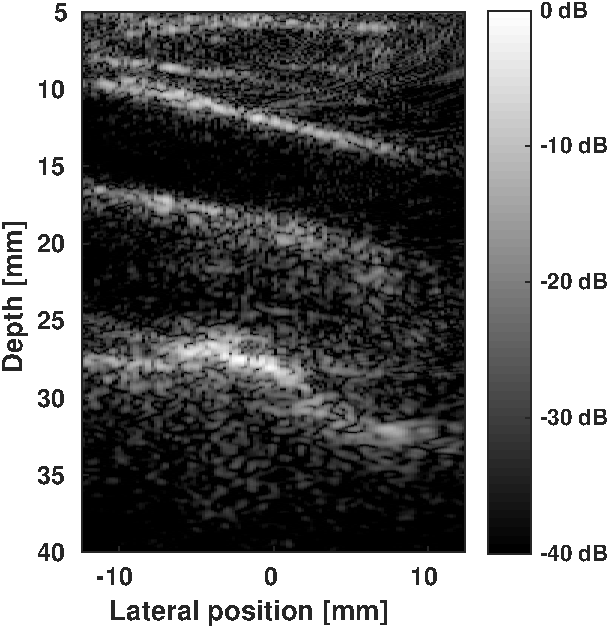
\includegraphics[height=\CarotidFigHeight]{figures/CS_carotid.pdf}}\hfill%
	\caption{B-mode image of an \textit{in vivo} carotid reconstructed with (a) \SI{100}{\percent} of the data and (b) \SI{25}{\percent} of the data acquired with the US-CMUX architecture.}
	\label{fig:carotid}
\end{figure} 
\newpage
\begin{table}[htb]
	\caption{Average values of the SNR~(\si{\decibel}) and SSIM over 10 draws for the different images, for $L = 2$ and $L = 4$.}
	\label{tab:SNR_SSIM}
	\centering
	\begin{tabular}{|c |c c|}
		\hline
		& Hyperechoic inclusion & \textit{In-vivo} carotid\\
		\hline
		SNR - $L = 2$ & $39$ & $36$\\
		SSIM - $L = 2$ & $0.94$ & $0.87$\\
		SNR - $L = 4$ & $32$ & $29$ \\
		SSIM - $L = 4$ & $0.81$ & $0.72$\\
		\hline
	\end{tabular}
\end{table} 


\bibliographystyle{IEEEtran}
% argument is your BibTeX string definitions and bibliography database(s)
\bibliography{SPARS2017}
%
% <OR> manually copy in the resultant .bbl file
% set second argument of \begin to the number of references
% (used to reserve space for the reference number labels box)




% that's all folks
\end{document}


